\let\negmedspace\undefined
\let\negthickspace\undefined
\documentclass[journal,12pt,onecolumn]{IEEEtran}
\usepackage{cite}
\usepackage{amsmath,amssymb,amsfonts,amsthm}
\usepackage{algorithmic}
\usepackage{graphicx}
\graphicspath{{./figs/}}
\usepackage{textcomp}
\usepackage{xcolor}
\usepackage{txfonts}
\usepackage{listings}
\usepackage{enumitem}
\usepackage{mathtools}
\usepackage{gensymb}
\usepackage{comment}
\usepackage{caption}
\usepackage[breaklinks=true]{hyperref}
\usepackage{tkz-euclide} 
\usepackage{listings}
\usepackage{gvv}                                        
%\def\inputGnumericTable{}                                 
\usepackage[latin1]{inputenc}     
\usepackage{xparse}
\usepackage{color}                                            
\usepackage{array}                                            
\usepackage{longtable}                                       
\usepackage{calc}                                             
\usepackage{multirow}
\usepackage{multicol}
\usepackage{hhline}                                           
\usepackage{ifthen}                                           
\usepackage{lscape}
\usepackage{tabularx}
\usepackage{array}
\usepackage{float}
\newtheorem{theorem}{Theorem}[section]
\newtheorem{problem}{Problem}
\newtheorem{proposition}{Proposition}[section]
\newtheorem{lemma}{Lemma}[section]
\newtheorem{corollary}[theorem]{Corollary}
\newtheorem{example}{Example}[section]
\newtheorem{definition}[problem]{Definition}
\newcommand{\BEQA}{\begin{eqnarray}}
\newcommand{\EEQA}{\end{eqnarray}}
\newcommand{\define}{\stackrel{\triangle}{=}}
\theoremstyle{remark}
\newtheorem{rem}{Remark}

\begin{document}

\title{
ASSIGNMENT 2: GATE 2014 \\
IN: INSTRUMENTATION ENGINEERING}
\author{EE25BTECH11062 - Vivek K Kumar}
\date{}
\maketitle

\begin{enumerate}

    \item Choose the most appropriate word from the options given below to complete the following sentence.\\

    
    A person suffering from Alzheimer's disease \underline{\hspace{2cm}} short-term memory loss.
   
    \hfill{\brak{\text{GATE IN 2014}}}
    \begin{enumerate}
    \begin{multicols}{2}
            \item experienced
            \item has experienced
            \item is experiencing
            \item experiences
    \end{multicols}
    \end{enumerate}

    \item Choose the most appropriate word from the options given below to complete the following sentence. \\
    \underline{\hspace{2cm}} is the key to their happiness; they are satisfied with what they have.

    \hfill{\brak{\text{GATE IN 2014}}}
        \begin{enumerate}
    \begin{multicols}{4}
            \item Contentment
            \item Ambition
            \item Perseverance
            \item Hunger
    \end{multicols}
        \end{enumerate}

    \item Which of the following options is the closest in meaning to the sentence below? \\
    "As a woman, I have no country."

    \hfill{\brak{\text{GATE IN 2014}}}
    \begin{enumerate}
        \item Women have no country.
        \item Women are not citizens of any country.
        \item Women's solidarity knows no national boundaries.
        \item Women of all countries have equal legal rights.
    \end{enumerate}

    \item In any given year, the probability of an earthquake of Magnitude 6 occurring in the Garhwal Himalayas is 0.04. The average time between successive occurrences of such earthquakes is \underline{\hspace{2cm}} years.

    \hfill{\brak{\text{GATE IN 2014}}}

    
    
    \item The population of a new city is 5 million and is growing at 20\% annually. How many years would it take to double at this growth rate?

    \hfill{\brak{\text{GATE IN 2014}}}
        \begin{enumerate}
    \begin{multicols}{4}
            \item 3-4 years
            \item 4-5
            \item 5-6 years
            \item 6-7 years
    \end{multicols}
        \end{enumerate}

\end{enumerate}

\begin{enumerate}
\setcounter{enumi}{5}

    \item In a group of four children, Som is younger to Riaz. Shiv is elder to Ansu. Ansu is youngest in the group. Which of the following statements is/are required to find the eldest child in the group? \\
    1. Shiv is younger to Riaz. \\
    2. Shiv is elder to Som.

    \hfill{\brak{\text{GATE IN 2014}}}
    \begin{enumerate}
        \item Statement 1 by itself determines the eldest child.
        \item Statement 2 by itself determines the eldest child.
        \item Statements 1 and 2 are both required to determine the eldest child.
        \item Statements 1 and 2 are not sufficient to determine the eldest child.
    \end{enumerate}

    
    
    \item Moving into a world of big data will require us to change our thinking about the merits of exactitude. To apply the conventional mindset of measurement to the digital, connected world of the twenty-first century is to miss a crucial point. As mentioned earlier, the obsession with exactness is an artefact of the information-deprived analog era. When data was sparse, every data point was critical, and thus great care was taken to avoid letting any point bias the analysis. \\
    From "BIG DATA" Viktor Mayer-Schonberger and Kenneth Cukier \\
    The main point of the paragraph is:

    \hfill{\brak{\text{GATE IN 2014}}}
    \begin{enumerate}
        \item The twenty-first century is a digital world
        \item Big data is obsessed with exactness
        \item Exactitude is not critical in dealing with big data
        \item Sparse data leads to a bias in the analysis
    \end{enumerate}

    \item The total exports and revenues from the exports of a country are given in the two pie charts below. The pie chart for exports shows the quantity of each item as a percentage of the total quantity of exports. The pie chart for the revenues shows the percentage of the total revenue generated through export of each item. The total quantity of exports of all the items is 5 lakh tonnes and the total revenues are 250 crore rupees. What is the ratio of the revenue generated through export of Item 1 per kilogram to the revenue generated through export of Item 4 per kilogram?

    \hfill{\brak{\text{GATE IN 2014}}}
    \begin{figure}[H]
        \centering
        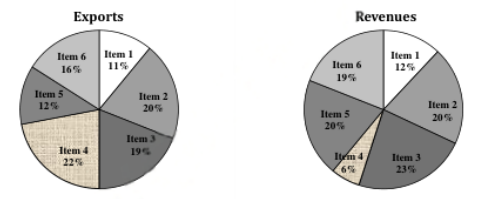
\includegraphics[width=0.8\columnwidth]{q8}
        \caption*{}
        \label{fig:q8}
    \end{figure}
        \begin{enumerate}
    \begin{multicols}{4}
            \item $1\colon2$
            \item $2\colon1$
            \item $1\colon4$
            \item $4\colon1$
    \end{multicols}
        \end{enumerate}

    \item X is 1 km northeast of Y. Y is 1 km southeast of Z. W is 1 km west of Z. P is 1 km south of W. Q is 1 km east of P. What is the distance between X and Q in km?

    \hfill{\brak{\text{GATE IN 2014}}}
        \begin{enumerate}
    \begin{multicols}{4}
            \item 1
            \item $\sqrt{2}$
            \item $\sqrt{3}$
            \item 2
    \end{multicols}
        \end{enumerate}
    
    \item 10\% of the population in a town is HIV+. A new diagnostic kit for HIV detection is available; this kit correctly identifies HIV+ individuals 95\% of the time, and HIV- individuals 89\% of the time. A particular patient is tested using this kit and is found to be positive. The probability that the individual is actually positive is \underline{\hspace{2cm}}.

    \hfill{\brak{\text{GATE IN 2014}}}

\end{enumerate}

\clearpage

\begin{enumerate}
    \item Given $x\brak{t} = 3 \sin\brak{1000 \pi t}$ and $y\brak{t} = 5 \cos\brak{1000 \pi t + \frac{\pi}{4}}$. The x-y plot will be

    \hfill{\brak{\text{GATE IN 2014}}}
        \begin{enumerate}
    \begin{multicols}{2}
            \item a circle
            \item a multi-loop closed curve
            \item a hyperbola
            \item an ellipse
            
    \end{multicols}
        \end{enumerate}
    
    \item Given that x is a random variable in the range $[0, \infty]$ with a probability density function $\frac{e^{-x/2}}{K}$, the value of the constant K is \underline{\hspace{2cm}}.

    \hfill{\brak{\text{GATE IN 2014}}}

    
    
    \item The figure shows the plot of y as a function of x.
    \begin{figure}[H]
        \centering
        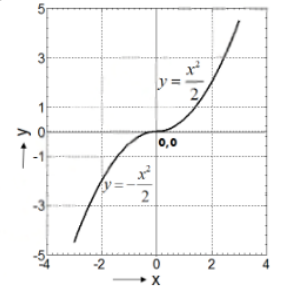
\includegraphics[width=0.5\columnwidth]{q3}
        \caption*{}
        \label{fig:q3}
    \end{figure}
    The function shown is the solution of the differential equation \brak{\text{assuming all initial conditions to be zero}} is:

    \hfill{\brak{\text{GATE IN 2014}}}
        \begin{enumerate}
    \begin{multicols}{4}
            \item $\frac{d^2y}{dx^2} = 1$
            \item $\frac{dy}{dx} = x$
            \item $\frac{dy}{dx} = -x$
            \item $\frac{dy}{dx} = \abs{x}$
    \end{multicols}
        \end{enumerate}

    \item A vector is defined as $\mathbf{f} = y\hat{i} + x\hat{j} + z\hat{k}$ where $\hat{i}, \hat{j}$ and $\hat{k}$ are unit vectors in Cartesian \brak{x,y,z} coordinate system. The surface integral $\oint_S \mathbf{f} \cdot d\mathbf{s}$ over the closed surface S of a cube with vertices having the following coordinates: \brak{0,0,0}, \brak{1,0,0}, \brak{1,1,0}, \brak{0,1,0}, \brak{0,0,1}, \brak{1,0,1}, \brak{1,1,1}, \brak{0,1,1} is \underline{\hspace{2cm}}.

    \hfill{\brak{\text{GATE IN 2014}}}

    

    \item The figure shows the schematic of a production process with machines A, B and C. An input job needs to be pre-processed either by A or by B before it is fed to C, from which the final finished product comes out. The probabilities of failure of the machines are given as: $P_A = 0.15$, $P_B = 0.05$, $P_C = 0.1$.
    \begin{figure}[H]
        \centering
        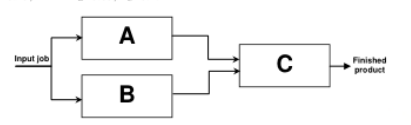
\includegraphics[width=0.4\columnwidth]{q5}
        \caption*{}
        \label{fig:q5}
    \end{figure}
    Assuming independence of failures of the machines, the probability that a given job is successfully processed \brak{\text{up to the third decimal place}} is \underline{\hspace{2cm}}.

    \hfill{\brak{\text{GATE IN 2014}}}

    

    \item The circuit shown in figure was at steady state for $t < 0$ with the switch at position 'A'. The switch is thrown to position 'B' at time $t = 0$. The voltage V \brak{\text{volts}} across the 10 $\ohm$ resistor at time $t=0^+$ is \underline{\hspace{2cm}}.
    \begin{figure}[H]
        \centering
        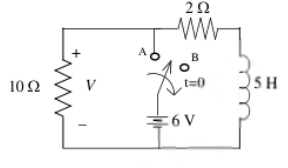
\includegraphics[width=0.4\columnwidth]{q6}
        \caption*{}
        \label{fig:q6}
    \end{figure}

    \hfill{\brak{\text{GATE IN 2014}}}

    \item The average real power in watts delivered to a load impedance $Z_L = \brak{4 - j2}\ohm$ by an ideal current source $i\brak{t} = 4 \sin\brak{\ohm t + 20\degree} A$ is \underline{\hspace{2cm}}.

    \hfill{\brak{\text{GATE IN 2014}}}

    
    
    \item Time domain expressions for the voltage $v_1\brak{t}$ and $v_2\brak{t}$ are given as $v_1\brak{t} = V_m \sin\brak{10t - 130\degree}$ and $v_2\brak{t} = V_m \cos\brak{10t + 10\degree}$.
    
    \hfill{\brak{\text{GATE IN 2014}}}
        \begin{enumerate}
    \begin{multicols}{2}
            \item $v_1\brak{t}$ leads $v_2\brak{t}$ by $130\degree$
            \item $v_1\brak{t}$ lags $v_2\brak{t}$ by $130\degree$
            \item $v_1\brak{t}$ lags $v_2\brak{t}$ by $-130\degree$
            \item $v_1\brak{t}$ leads $v_2\brak{t}$ by $-130\degree$
    \end{multicols}
        \end{enumerate}

    \item A pH electrode obeys Nernst equation and is being operated at $25\degree C$. The change in the open circuit voltage in millivolts across the electrode for a pH change from 6 to 8 is \underline{\hspace{2cm}}.

    \hfill{\brak{\text{GATE IN 2014}}}

    
    
    \item The pressure and velocity at the throat of a Venturi tube, measuring the flow of a liquid, are related to the upstream pressure and velocity, respectively, as follows:

    \hfill{\brak{\text{GATE IN 2014}}}
    \begin{enumerate}
        \item pressure is lower but velocity is higher
        \item pressure is higher but velocity is lower
        \item both pressure and velocity are lower
        \item pressure and velocity are identical
    \end{enumerate}

    
    
    \item Semiconductor strain gages typically have much higher gage factors than those of metallic strain gages, primarily due to:

    \hfill{\brak{\text{GATE IN 2014}}}
    \begin{enumerate}
        \item higher temperature sensitivity
        \item higher Poisson's ratio
        \item higher piezoresistive coefficient
        \item higher magnetostrictive coefficient
    \end{enumerate}

    
    
    \item For a rotameter, which one of the following statements is TRUE?

    \hfill{\brak{\text{GATE IN 2014}}}
    \begin{enumerate}
        \item the weight of the float is balanced by the buoyancy and the drag force acting on the float
        \item the velocity of the fluid remains constant for all positions of the float
        \item the measurement of volume flow rate of gas is not possible
        \item the volume flow rate is insensitive to changes in density of the fluid
    \end{enumerate}

    
    
    \item For the op-amp shown in the figure, the bias currents are $I_{b1} = 450$ nA and $I_{b2} = 350$ nA. The values of the input bias current \brak{I_B} and the input offset current \brak{I_f} are:
    \begin{figure}[H]
        \centering
        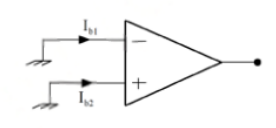
\includegraphics[width=0.3\columnwidth]{q13}
        \caption*{}
        \label{fig:q13}
    \end{figure}

    \hfill{\brak{\text{GATE IN 2014}}}
        \begin{enumerate}
    \begin{multicols}{2}
            \item $I_B = 800$ nA, $I_f = 50$ nA
            \item $I_B = 800$ nA, $I_f = 100$ nA
            \item $I_B = 400$ nA, $I_f = 50$ nA
            \item $I_B = 400$ nA, $I_f = 100$ nA
    \end{multicols}
        \end{enumerate}
    
    \item The amplifier in the figure has gain of -10 and input resistance of 50 k$\ohm$. The values of $R_i$ and $R_f$ are:
    \begin{figure}[H]
        \centering
        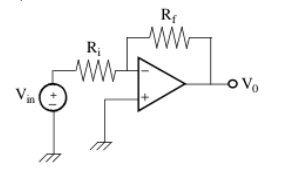
\includegraphics[width=0.4\columnwidth]{q14}
        \caption*{}
        \label{fig:q14}
    \end{figure}

    \hfill{\brak{\text{GATE IN 2014}}}
        \begin{enumerate}
    \begin{multicols}{2}
            \item $R_i = 500$ k$\ohm$, $R_f = 50$ k$\ohm$
            \item $R_i = 50$ k$\ohm$, $R_f = 500$ k$\ohm$
            \item $R_i = 5$ k$\ohm$, $R_f = 10$ k$\ohm$
            \item $R_i = 50$ k$\ohm$, $R_f = 200$ k$\ohm$
    \end{multicols}
        \end{enumerate}
    
    \item For the circuit shown in the figure assume ideal diodes with zero forward resistance and zero forward voltage drop. The current through the diode $D_2$ in mA is \underline{\hspace{2cm}}.
    \begin{figure}[H]
        \centering
        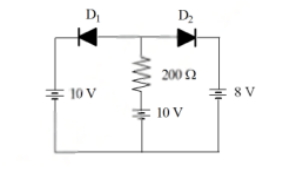
\includegraphics[width=0.4\columnwidth]{q15}
        \caption*{}
        \label{fig:q15}
    \end{figure}
    \hfill{\brak{\text{GATE IN 2014}}}
    
    \item The system function of an LTI system is given by $H\brak{z} = \frac{1 - \frac{1}{3}z^{-1}}{1 - \frac{1}{4}z^{-1}}$. The above system can have stable inverse if the region of convergence of H\brak{z} is defined as

    \hfill{\brak{\text{GATE IN 2014}}}
        \begin{enumerate}
    \begin{multicols}{4}
            \item $|z| > \frac{1}{3}$
            \item $|z| < \frac{1}{12}$
            \item $|z| > \frac{1}{4}$
            \item $|z| < \frac{1}{3}$
    \end{multicols}
        \end{enumerate}
    
    \item The figure is a logic circuit with inputs A and B and output Y. Vss = +5V. The circuit is of type
    \begin{figure}[H]
        \centering
        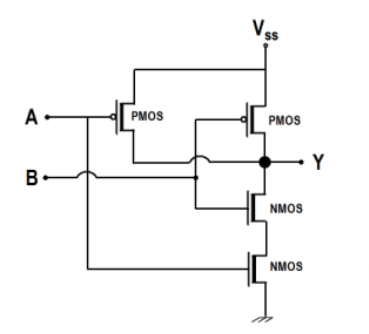
\includegraphics[width=0.4\columnwidth]{q17}
        \caption*{}
        \label{fig:q17}
    \end{figure}

    \hfill{\brak{\text{GATE IN 2014}}}
        \begin{enumerate}
    \begin{multicols}{4}
            \item NOR
            \item AND
            \item OR
            \item NAND
    \end{multicols}
        \end{enumerate}

    \item The impulse response of an LTI system is given as:
    $h[n] = \frac{\sin\brak{\ohm_c n}}{\pi n}, n \neq 0$; $h[n] = \frac{\ohm_c}{\pi}, n=0$. It represents an ideal

    \hfill{\brak{\text{GATE IN 2014}}}
        \begin{enumerate}
    \begin{multicols}{2}
            \item non-causal, low-pass filter
            \item causal, low-pass filter
            \item non-causal, high-pass filter
            \item causal, high-pass filter
    \end{multicols}
        \end{enumerate}

    \item A discrete-time signal $x[n]$ is obtained by sampling an analog signal at 10 kHz. The signal $x[n]$ is filtered by a system with impulse response $h[n] = 0.5\{\delta[n] + \delta[n-1]\}$. The 3dB cutoff frequency of the filter is:

    \hfill{\brak{\text{GATE IN 2014}}}
        \begin{enumerate}
    \begin{multicols}{4}
            \item 1.25 kHz
            \item 2.50 kHz
            \item 4.00 kHz
            \item 5.00 kHz
    \end{multicols}
        \end{enumerate}

    \item A full duplex binary FSK transmission is made through a channel of bandwidth 10 kHz. In each direction of transmission the two carriers used for the two states are separated by 2 kHz. The maximum baud rate for this transmission is:

    \hfill{\brak{\text{GATE IN 2014}}}
        \begin{enumerate}
    \begin{multicols}{4}
            \item 2000 bps
            \item 3000 bps
            \item 5000 bps
            \item 10000 bps
    \end{multicols}
        \end{enumerate}
    
    \item A loop transfer function is given by: 
    \begin{align*}
    G\brak{s}H\brak{s} = \frac{K\brak{s+2}}{s^2\brak{s+10}}   
    \end{align*}
    The point of intersection of the asymptotes of $G\brak{s}H\brak{s}$ on the real axis in the s-plane is at \underline{\hspace{2cm}}.

    \hfill{\brak{\text{GATE IN 2014}}}
    
    \item The resistance and inductance of an inductive coil are measured using an AC bridge as shown in the figure. The bridge is to be balanced by varying the impedance Z2. For obtaining balance, Z2 should consist of element\brak{\text{s}}:
    \begin{figure}[H]
        \centering
        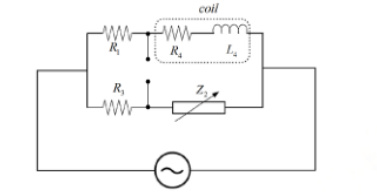
\includegraphics[width=0.6\columnwidth]{q22}
        \caption*{}
        \label{fig:q22}
    \end{figure}

    \hfill{\brak{\text{GATE IN 2014}}}
        \begin{enumerate}
    \begin{multicols}{4}
            \item R and C
            \item R and L
            \item L and C
            \item Only C
    \end{multicols}
        \end{enumerate}
    
    \item A plant has an open-loop transfer function, 
    \begin{align*}
    G_p\brak{s} = \frac{20}{\brak{s+0.1}\brak{s+2}\brak{s+100}}
    \end{align*}
    The approximate model obtained by retaining only one of the above poles, which is closest to the frequency response of the original transfer function at low frequency is

    \hfill{\brak{\text{GATE IN 2014}}}
        \begin{enumerate}
    \begin{multicols}{4}
            \item $\frac{0.1}{s+0.1}$
            \item $\frac{2}{s+2}$
            \item $\frac{100}{s+100}$
            \item $\frac{20}{s+0.1}$
    \end{multicols}
        \end{enumerate}

    \item In order to remove respiration related motion artifacts from an ECG signal, the following filter should be used:

    \hfill{\brak{\text{GATE IN 2014}}}
    \begin{enumerate}
        \item low-pass filter with $f_c = 0.5$ Hz
        \item high-pass filter with $f_c = 0.5$ Hz
        \item high-pass filter with $f_c = 49.5$ Hz
        \item band-pass filter with passband between 0.1 Hz and 0.5 Hz
    \end{enumerate}
    
    \item In a time-of-flight mass spectrometer if $q$ is the charge and $m$ the mass of the ionized species, then the time of flight is proportional to

    \hfill{\brak{\text{GATE IN 2014}}}
        \begin{enumerate}
    \begin{multicols}{4}
            \item $\frac{\sqrt{m}}{\sqrt{q}}$
            \item $\frac{\sqrt{q}}{\sqrt{m}}$
            \item $\frac{m}{\sqrt{q}}$
            \item $\frac{q}{\sqrt{m}}$
    \end{multicols}
        \end{enumerate}

\end{enumerate}

\clearpage
\begin{enumerate}
\setcounter{enumi}{25}
    \item A scalar valued function is defined as $f\brak{\mathbf{x}} = \mathbf{x}^T A \mathbf{x} + \mathbf{b}^T \mathbf{x}$, where A is a symmetric positive definite matrix with dimension $n \times n$; b and x are vectors of dimension $n \times 1$. The minimum value of $f\brak{\mathbf{x}}$ will occur when $\mathbf{x}$ equals
    
    \hfill{\brak{\text{GATE IN 2014}}}
        \begin{enumerate}
    \begin{multicols}{2}
            \item $\brak{A^T A}^{-1} b$
            \item $-\brak{A^T A}^{-1} b$
            \item $-\frac{1}{2} A^{-1} b$
            \item $\frac{1}{2} A^{-1} b$
    \end{multicols}
        \end{enumerate}

    \item The iteration step in order to solve for the cube roots of a given number N using the Newton Raphson's method

    \hfill{\brak{\text{GATE IN 2014}}}
        \begin{enumerate}
    \begin{multicols}{2}
            \item $x_{k+1} = x_k + \frac{1}{3}\brak{x_k^3 - N}$
            \item $x_{k+1} = \frac{1}{2} \brak{ x_k + \frac{N}{x_k^2}}$
            \item $x_{k+1} = x_k - \frac{1}{3}\brak{x_k^3 - N}$
            \item $x_{k+1} = \frac{1}{2} \brak{ x_k - \frac{N}{x_k^2} }$
    \end{multicols}
        \end{enumerate}
    
    \item For the matrix A satisfying the equation given below, the eigenvalues are
    \begin{align*}
        \myvec{A}\myvec{1 & 2 & 3 \\ 4 & 5 & 6 \\ 7 & 8 & 9}
         = \myvec{1 & 2 & 3 \\ 4 & 5 & 6 \\ 7 & 8 & 9 }
    \end{align*}

    \hfill{\brak{\text{GATE IN 2014}}}
        \begin{enumerate}
    \begin{multicols}{2}
            \item \brak{1, j, -j}
            \item \brak{1, 1, 0}
            \item \brak{1, 1, -1}
            \item \brak{1, 0, 0}
    \end{multicols}
        \end{enumerate}
    
    \item In the circuit shown in the figure, initially the capacitor is uncharged. The switch 'S' is closed at $t=0$. Two milliseconds after the switch is closed, the current through the capacitor \brak{\text{in mA}} is \underline{\hspace{2cm}}.
    \begin{figure}[H]
        \centering
        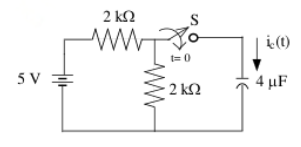
\includegraphics[width=0.4\columnwidth]{q29}
        \caption*{}
        \label{fig:q29}
    \end{figure}

    \hfill{\brak{\text{GATE IN 2014}}}
    
    \item A capacitor 'C' is to be connected across the terminals 'A' and 'B' as shown in the figure so that the power factor of the parallel combination becomes unity. The value of the capacitance required in $\mu$F is \underline{\hspace{2cm}}.
    \begin{figure}[H]
        \centering
        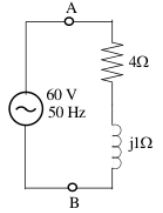
\includegraphics[width=0.4\columnwidth]{q30}
        \caption*{}
        \label{fig:q30}
    \end{figure}

    \hfill{\brak{\text{GATE IN 2014}}}
    
    \item The resistance of a wire is given by the expression $R = \frac{4\rho L}{\pi D^2}$, where, $\rho$ is the resistivity \brak{\ohm}-meter, L is the length \brak{\text{meter}} and D \brak{\text{meter}} is the diameter of the wire. The error in measurement of each of the parameters $\rho$, L, and D is $\pm1.0\%$. Assuming that the errors are independent random variables, the percent error in measurement of R is \underline{\hspace{2cm}}.

    \hfill{\brak{\text{GATE IN 2014}}}

    
    
    \item The circuit shown in the figure contains a dependent current source between A and B terminals. The Thevenin's equivalent resistance in k$\ohm$ between the terminals C and D is \underline{\hspace{2cm}}.
    \begin{figure}[H]
        \centering
        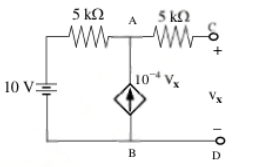
\includegraphics[width=0.5\columnwidth]{q32}
        \caption*{}
        \label{fig:q32}
    \end{figure}

    \hfill{\brak{\text{GATE IN 2014}}}
    \item A thermistor has a resistance of 1 k$\ohm$ at temperature 298 K and 465 $\ohm$ at temperature 316 K. The temperature sensitivity in K$^{-1}$ [i.e. \brak{1/R}\brak{dR/dT}, where R is the resistance at the temperature T \brak{\text{in K}}], of this thermistor at 316 K is \underline{\hspace{2cm}}.

    \hfill{\brak{\text{GATE IN 2014}}}

    
    
    \item A barium titanate piezoelectric crystal with $d_{33} = 150$ pC/N, $C_{crystal} = 25$ pF and $R_{crystal} = 10^{10} \ohm$ is used to measure the amplitude of a step force. The voltage output is measured using a digital voltmeter with input impedance $10^{13} \ohm$ connected across the crystal. All other capacitances and resistances may be neglected. A step force of 2 N is applied from direction "3" on the crystal. The time in milliseconds within which the voltmeter should sample the crystal output voltage so that the drop from the peak value is no more than 0.12V is \underline{\hspace{2cm}}.

    \hfill{\brak{\text{GATE IN 2014}}}

    
    
    \item A thermopile is constructed using 10 junctions of Chromel-Constantan \\ \brak{\text{sensitivity $60\mu V/\degree C$ for each junction}} connected in series. The output is fed to an amplifier having an infinite input impedance and a gain of 10. The output from the amplifier is acquired using a 10-bit ADC, with reference voltage of 5 V. The resolution of this system in units of $\degree C$ is \underline{\hspace{2cm}}.

    \hfill{\brak{\text{GATE IN 2014}}}

    

    \item A transit time ultrasonic flowmeter uses a pair of ultrasonic transducers placed at 45$\degree$ angle, as shown in the figure. The inner diameter of the pipe is 0.5 m. The differential transit time is directly measured using a clock of frequency 5 MHz. The velocity of the fluid is small compared to the velocity of sound in the static fluid, which is 1500 m/s and the size of the crystals is negligible compared to the diameter of the pipe. The minimum change in fluid velocity \brak{\text{m/s}} that can be measured using this system is \underline{\hspace{2cm}}.
    \begin{figure}[H]
        \centering
        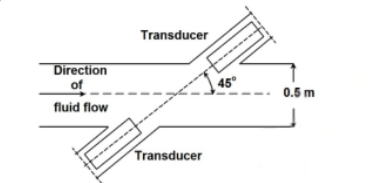
\includegraphics[width=0.6\columnwidth]{q36}
        \caption*{}
        \label{fig:q36}
    \end{figure}

    \hfill{\brak{\text{GATE IN 2014}}}
    
    \item Assuming an ideal op-amp in linear range of operation, the magnitude of the transfer impedance $\frac{v_0}{i}$ in M$\ohm$ of the current to voltage converter shown in the figure is \underline{\hspace{2cm}}.
    \begin{figure}[H]
        \centering
        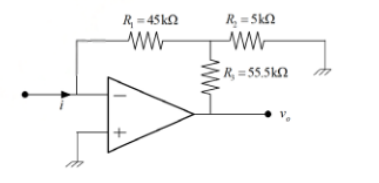
\includegraphics[width=0.6\columnwidth]{q37}
        \caption*{}
        \label{fig:q37}
    \end{figure}

    \hfill{\brak{\text{GATE IN 2014}}}
    
    \item For the circuit shown in the figure, the transistor has $\beta = 40$, $V_{BE} = 0.7$ V, and the voltage across the Zener diode is 15 V. The current \brak{\text{in mA}} through the Zener diode is \underline{\hspace{2cm}}.
    \begin{figure}[H]
        \centering
        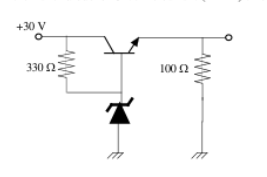
\includegraphics[width=0.4\columnwidth]{q38}
        \caption*{}
        \label{fig:q38}
    \end{figure}

    \hfill{\brak{\text{GATE IN 2014}}}

    \item In the figure, transistors T1 and T2 have identical characteristics. $V_{CE\brak{sat}}$ of transistor T3 is 0.1 V. The voltage $V_1$ is high enough to put T3 in saturation. Voltage $V_{BE}$ of transistors T1, T2 and T3 is 0.7 V. The value of \brak{V_1 - V_2} in V is \underline{\hspace{2cm}}.
    \begin{figure}[H]
        \centering
        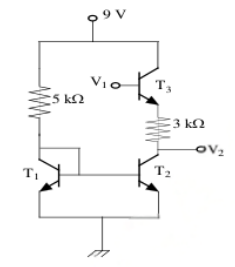
\includegraphics[width=0.4\columnwidth]{q39}
        \caption*{}
        \label{fig:q39}
    \end{figure}

    \hfill{\brak{\text{GATE IN 2014}}}

    \item The figures show an oscillator circuit having an ideal Schmitt trigger and its input-output characteristics. The time period \brak{\text{in ms}} of $v_o\brak{t}$ is \underline{\hspace{2cm}}.
    \begin{figure}[H]
        \centering
        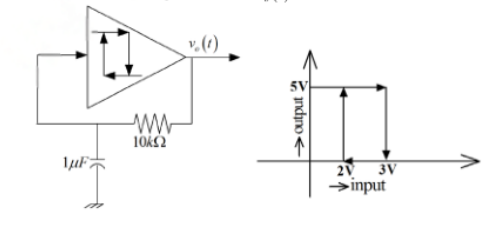
\includegraphics[width=0.55\columnwidth]{q40}
        \caption*{}
        \label{fig:q40}
    \end{figure}

    \hfill{\brak{\text{GATE IN 2014}}}
    
    \item An N-bit ADC has an analog reference voltage V. Assuming zero mean and uniform distribution of the quantization error, the quantization noise power will be:

    \hfill{\brak{\text{GATE IN 2014}}}
        \begin{enumerate}
    \begin{multicols}{2}
            \item $\frac{V^2}{12\brak{2^N-1}^2}$
            \item $\frac{V^2}{12\brak{2^N-1}}$
            \item $\frac{V}{12\brak{2^N-1}}$
            \item $\frac{V^2}{\sqrt{12}}$
    \end{multicols}
        \end{enumerate}
    
    \item A microprocessor accepts external interrupts \brak{\text{Ext INT}} through a Programmable Interrupt Controller as shown in the figure. Assuming vectored interrupt, a correct sequence of operations when a single external interrupt \brak{\text{Ext INT1}} is received will be:
    \begin{figure}[H]
        \centering
        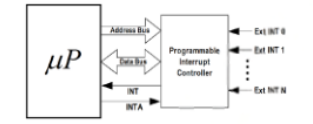
\includegraphics[width=0.6\columnwidth]{q42}
        \caption*{}
        \label{fig:q42}
    \end{figure}

    \hfill{\brak{\text{GATE IN 2014}}}
    \begin{enumerate}
        \item Ext INT1 $\rightarrow$ INTA $\rightarrow$ Data Read $\rightarrow$ INT
        \item Ext INT1 $\rightarrow$ INT $\rightarrow$ INTA $\rightarrow$ Data Read
        \item Ext INT1 $\rightarrow$ INT $\rightarrow$ INTA $\rightarrow$ Address Write
        \item Ext INT1 $\rightarrow$ INT $\rightarrow$ Data Read $\rightarrow$ Address Write
    \end{enumerate}

    

    \item The circuit in the figure represents a counter-based unipolar ADC. When SOC is asserted the counter is reset and clock is enabled so that the counter counts up and the DAC output grows. When the DAC output exceeds the input sample value, the comparator switches from logic 0 to logic 1, disabling the clock and enabling the output buffer by asserting EOC. Assuming all components to be ideal, $V_{ref}$, DAC output and input to be positive, the maximum error in conversion of the analog sample value is:
    \begin{figure}[H]
        \centering
        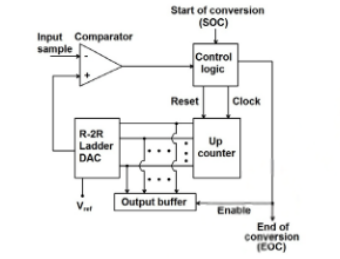
\includegraphics[width=0.6\columnwidth]{q43}
        \caption*{}
        \label{fig:q43}
    \end{figure}

    \hfill{\brak{\text{GATE IN 2014}}}
    \begin{enumerate}
    \begin{multicols}{2}
        \item directly proportional to $V_{ref}$
        \item inversely proportional to $V_{ref}$
        \item independent of $V_{ref}$
        \item directly proportional to clock frequency
    \end{multicols}
    \end{enumerate}

    

    \item $X\brak{k}$ is the Discrete Fourier Transform of a 6-point real sequence $x\brak{n}$. If $X\brak{0} = 9+j0, X\brak{2} = 2+j2, X\brak{3} = 3-j0, X\brak{5} = 1-j1$, then $x\brak{0}$ is

    \hfill{\brak{\text{GATE IN 2014}}}
        \begin{enumerate}
    \begin{multicols}{4}
            \item 3
            \item 9
            \item 15
            \item 18
    \end{multicols}
        \end{enumerate}

    \item The transfer function of a digital system is given by: 
    \begin{align*}
    \frac{b_0}{1 - az^{-1} + 2z^{-2}}; \text{where $a_2$ is real}
    \end{align*}
    The transfer function is BIBO stable if the value of $a_2$ is:

    \hfill{\brak{\text{GATE IN 2014}}}
        \begin{enumerate}
    \begin{multicols}{4}
            \item -1.5
            \item -0.75
            \item 0.5
            \item 1.5
    \end{multicols}
        \end{enumerate}

    \item The transfer function of a system is given by 
    \begin{align*}
    G\brak{s} = \frac{e^{-s/500}}{s+500}
    \end{align*}
    The input to the system is $x\brak{t} = \sin\brak{100\pi t}$. In periodic steady state the output of the system is found to be $y\brak{t} = A\sin\brak{100\pi t - \phi}$. The phase angle \brak{\phi} in degree is \underline{\hspace{2cm}}.

    \hfill{\brak{\text{GATE IN 2014}}}

    
    
    \item In the microprocessor controlled measurement scheme shown in the figure, $R_x$ is the unknown resistance to be measured, while $R_{ref}$ and $C_{ref}$ are known. $C_{ref}$ is charged from voltage $V_L$ to $V_H$ \brak{\text{by a constant DC voltage source $V_S$}}, once through $R_{ref}$ in $T_{ref}$ seconds and then discharged to $V_L$. It is again charged from voltage $V_L$ to $V_H$ through $R_x$ in $T_x$ seconds. If $T_x = k T_{ref}$ then
    \begin{figure}[H]
        \centering
        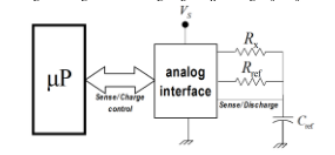
\includegraphics[width=0.6\columnwidth]{q47}
        \caption*{}
        \label{fig:q47}
    \end{figure}

    \hfill{\brak{\text{GATE IN 2014}}}
        \begin{enumerate}
    \begin{multicols}{2}
            \item $R_x = kR_{ref} \brak{1 - \frac{V_L}{V_H}}$
            \item $R_x = kR_{ref} \ln\brak{\frac{V_H}{V_L}}$
            \item $R_x = kR_{ref}$
            \item $R_x = \ln\brak{k} R_{ref}$
    \end{multicols}
        \end{enumerate}

    \item Frequency of an analog periodic signal in the range of 5kHz - 10kHz is to be measured with a resolution of 100Hz by measuring its period with a counter. Assuming negligible signal and transition delays the minimum clock frequency and minimum number of bits in the counter needed, respectively, are:

    \hfill{\brak{\text{GATE IN 2014}}}
        \begin{enumerate}
    \begin{multicols}{2}
            \item 1 MHz, 10-bits
            \item 10 MHz, 10-bits
            \item 1 MHz, 8-bits
            \item 10MHz, 8-bits
    \end{multicols}
        \end{enumerate}

    \item The loop transfer function of a feedback control system is given by 
    \begin{align*}
        G\brak{s}H\brak{s} = \frac{1}{s\brak{s+1}\brak{9s+1}}
    \end{align*}
    Its phase crossover frequency \brak{\text{in rad/s}}, approximated to two decimal places, is \underline{\hspace{2cm}}.

    \hfill{\brak{\text{GATE IN 2014}}}

    
    
    \item Consider a transport lag process with a transfer function 
    \begin{align*}
    G_p\brak{s} = e^{-s}
    \end{align*}
    The process is controlled by a purely integral controller with transfer function 
    \begin{align*}
    G_c\brak{s} = \frac{K_i}{s}
    \end{align*}
    in a unity feedback configuration. The value of $K_i$ for which the closed loop plant has a pole at $s = -1$, is \underline{\hspace{2cm}}.

    \hfill{\brak{\text{GATE IN 2014}}}

    

    \item Consider the control system shown in figure with feedforward action for rejection of a measurable disturbance $d\brak{t}$. The value of K, for which the disturbance response at the output $y\brak{t}$ is zero mean, is:
    \begin{figure}[H]
        \centering
        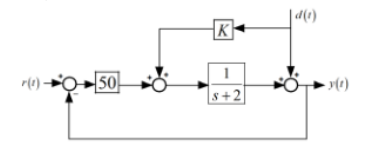
\includegraphics[width=0.62\columnwidth]{q51}
        \caption*{}
        \label{fig:q51}
    \end{figure}

    \hfill{\brak{\text{GATE IN 2014}}}
        \begin{enumerate}
    \begin{multicols}{4}
            \item 1
            \item -1
            \item 2
            \item -2
    \end{multicols}
        \end{enumerate}

    \item A mixture contains two mutually inert solutions 'X' and 'Y' in equal volumes. The mixture is examined in a spectrophotometer using a cuvette. It is observed that the transmittance is 0.40. With only the solution 'X' in the same cuvette, the transmittance is 0.20. With only solution 'Y' in the cuvette the transmittance is \underline{\hspace{2cm}}.

    \hfill{\brak{\text{GATE IN 2014}}}

    
    
    \item Monochromatic light from a step index \brak{n_1 = 1.500; n_2 = 1.485}, multimode optical fiber of core diameter 100 $\mu$m is incident through air \brak{n = 1.000} onto a linear photo-detector array placed at 1 mm distance from the tip of the fiber. The tip of the fiber is polished and its exit plane is perpendicular to the axis of the fiber. The detector array is oriented parallel to the exit plane of the tip. The array consists of photo-detector elements each of 5 $\mu$m diameter. The distance between the edges of two adjacent elements can be assumed to be zero. The number of elements illuminated by the light coming out of the fiber is \underline{\hspace{2cm}}.

    \hfill{\brak{\text{GATE IN 2014}}}

    
    
    \item An image of the chest of a patient is taken with an X-ray machine on a photographic film. The Hurter-Driffield \brak{\text{HD}} curve of the film is shown in the figure. The highly absorbing parts of the body \brak{\text{e.g. bones}}, show up as low exposure regions \brak{\text{mapped near A}} and the less absorbing parts \brak{\text{e.g. muscles}} show up as high exposure regions \brak{\text{mapped near B}}.
    \begin{figure}[H]
        \centering
        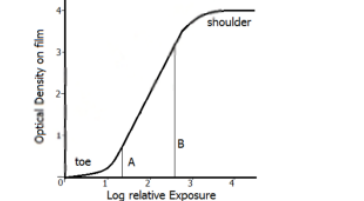
\includegraphics[width=0.5\columnwidth]{q54}
        \caption*{}
        \label{fig:q54}
    \end{figure}
    If the exposure time is increased 10 times, while keeping the voltages and currents in the X-ray machine constant, in the image,

    \hfill{\brak{\text{GATE IN 2014}}}
    \begin{enumerate}
        \item contrast decreases since B moves into the shoulder region
        \item contrast decreases since both A and B move into the shoulder region
        \item contrast increases since A moves into the toe region
        \item contrast decreases since both A and B move into the toe region
    \end{enumerate}

    

    \item
    \begin{figure}[H]
        \centering
        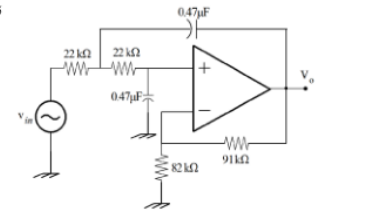
\includegraphics[width=0.6\columnwidth]{q55}
        \caption*{}
        \label{fig:q55}
    \end{figure}
    For the given low-pass circuit shown in the figure, the cutoff frequency in Hz will be \underline{\hspace{2cm}}.

    \hfill{\brak{\text{GATE IN 2014}}}
    
\end{enumerate}

\begin{center}
    \textbf{END OF THE QUESTION PAPER}
\end{center}

\end{document}
